% ======================================================================================
%  Appendix
% ======================================================================================
\section{Experimental setup}
\label{app:setup}

\paragraph{Encoders.} Foundation models (RETFound, MIRAGE, DINOv2) and CNNs (ResNet-50, ConvNeXt-T/B/L, the
98k-parameter SmallCNN) are frozen feature extractors with a linear head, or fine-tuned end-to-end (``FT'').
\emph{Linear probe:} \texttt{StandardScaler} + $\ell_2$ logistic regression, \texttt{LogisticRegressionCV}
($C\in\{0.01,0.05,0.2,1.0\}$, 3-fold, ROC-AUC, \texttt{max\_iter}=5000; small-$n$ fallback $C{=}0.05$), fit on clean
training eyes (seed-0). Features: DINOv2 = \texttt{[CLS]}\,$\oplus$\,mean patch tokens (registers excluded) at
$224^2$; RETFound = global-avg-pool + \texttt{fc\_norm} at $224^2$ (ImageNet normalization); MIRAGE = encoder last
token at native $512^2$ (unit-scaled, not ImageNet-normed); ResNet/ConvNeXt = global-avg-pool. \emph{Fine-tune:}
AdamW (weight decay 0.05), 50 epochs, batch 32, layer-wise LR decay (ConvNeXt 0.9 / ResNet 1.0 / ViT 0.65),
base-LR $5\times10^{-4}$/$10^{-3}$/$5\times10^{-3}$ linearly scaled by batch, warmup then cosine to $10^{-6}$,
class-weighted cross-entropy with label-smoothing 0.1, \texttt{RandomResizedCrop}(0.5--1.0)+HFlip+RandomErasing(0.25)
at $224^2$, mixed precision, early stop (patience 12) on validation AUC. \emph{SmallCNN} ($\sim$98k params):
four \texttt{Conv}$3{\times}3$--GroupNorm--ReLU--MaxPool blocks (16/32/64/128) $\rightarrow$ global-avg-pool
$\rightarrow$ linear logit; Adam ($10^{-3}$, wd $10^{-4}$), class-weighted BCE. It is trained end-to-end from scratch
on each scored axis (GLEAM B-scans; Harvard-GDP thickness maps), on the same seed-0 split as the other readers. It is
never exposed to the test shift.

\paragraph{VLMs.} All seven VLMs receive byte-identical eyes, shifts (per-eye seeds $3000{+}e$, $4000{+}e$), few-shot
exemplars (seed $+11$) and prompts from a single shared axis builder, are queried greedily (one
sample) for a verbalized probability \citep{tian2023calibration}, and are thresholded at the clean-data
90\%-specificity operating point. Exact model IDs and inference settings are in Table~\ref{tab:models}. The verbatim
prompts, few-shot construction and probability parsing are in App.~\ref{app:prompts}.

\paragraph{Statistics.} Confidence intervals are eye-level percentile bootstraps (2000 resamples; the eye is the
resampling unit) \citep{diciccio1996bootstrap}. ECE uses 10 equal-width confidence bins \citep{guo2017calibration}. The operating point (target specificity 0.90) is fixed on
clean negatives and reused on shifted scores; $\Delta$sens@spec and spec@shift are read there, while decision-flip
is the change in the fixed $0.5$ clinical call (refer / do-not-refer). Both capture decision movement at a
deployed threshold. Sample sizes: $n{=}360$ eyes (B-scan axis), $n{=}300$ eyes (thickness-map
axis).

\paragraph{Compute.} The open-weights VLMs and all fine-tuning run on a single Colab GPU (A100-40GB or L4), bf16,
\texttt{device\_map=auto}, batched greedy generation. The closed API configurations (Gemini, GPT-5.6 Sol, Claude) are CPU-only
clients. Reproducing the tables and figures from the released per-eye outputs requires no GPU.

\section{Prompts and elicitation}
\label{app:prompts}

Elicitation is a single verbalized referral probability per eye \citep{tian2023calibration}, the score common to
every vendor, since the closed models expose no logprobs. Prompts are byte-identical across models on a given axis.

\paragraph{B-scan axis.} System: \emph{``You are grading circumpapillary OCT B-scans for glaucoma. Each
image is a cross-sectional retinal scan taken in a ring around the optic nerve head. Glaucoma shows as thinning/loss
of the retinal nerve fibre layer (RNFL) and neuroretinal rim.''} Query: \emph{``Now assess THIS new B-scan. Return
JSON: \texttt{glaucoma\_referral\_probability} (0--1, your calibrated probability that this eye should be referred
for glaucoma), \texttt{rationale} (one short sentence).''}

\paragraph{Thickness-map axis.} System: \emph{``You are grading en-face retinal nerve fibre layer (RNFL) THICKNESS
MAPS for glaucoma. Each image is a colour-coded map of RNFL thickness around the optic disc: warm colours = THICK,
cool colours = THIN. Glaucoma shows as THINNING---loss of the bright superior and inferior nerve-fibre bundles (the
`double-hump'), a wedge defect or diffuse darkening.''} Query: as above with ``RNFL thickness map''.

\paragraph{Few-shot.} $k{=}6$ labeled exemplars, drawn only from the training pool (leakage guard), balanced:
B-scan axis severity-graded (3 healthy + one each early/moderate/advanced); map axis binary (3 glaucoma + 3
healthy). Selection RNG is \texttt{seed}$+11$ and the exemplar set is identical across models. The few-shot preamble
adds \emph{``Below are LABELLED reference images in this exact format so you can calibrate''}; each exemplar is
captioned with its label before (API/open configurations) or after (Gemini) its image.

\paragraph{Probability parsing.} We read \texttt{glaucoma\_referral\_probability} from the JSON (regex fallback on
the first such field, clipped to $[0,1]$); parse failures are retried (up to 5, exponential backoff) and, only if
still failing, imputed as 0.5 (never cached). Imputation is rare for the frontier configurations but non-negligible
for the small-model configurations that collapse to a near-constant output (e.g.\ Qwen3-VL-8B on the map), where it
biases ECE and AUC toward chance and reinforces the near-chance reading of those configurations. An alternative boolean-verdict schema
maps $p{=}\text{conf}$ if glaucoma else $1{-}\text{conf}$. We use the probability schema throughout for parity.

\begin{table}[t]
  \centering
  \caption{\textbf{Model card.} Exact identifiers, size and inference settings. VLMs are queried $N{=}1$,
  greedily. Reasoning/thinking is enabled where supported (``high''/dynamic). Temperature is omitted for the
  reasoning API models (they reject it) and set to 0 for Gemini.}
  \label{tab:models}
  \small
  \renewcommand{\arraystretch}{0.9}
  \setlength{\tabcolsep}{4pt}
  \begin{tabular}{lll}
    \toprule
    Model & Identifier & Params / settings \\
    \midrule
    \multicolumn{3}{l}{\textit{Vision-language models (prompted)}} \\
    \midrule
    Gemini 2.5 Flash / Pro & \texttt{gemini-2.5-flash}, \texttt{-pro} & temp 0, thinking budget \\
    Gemini 3.6 Flash & \texttt{gemini-3.6-flash} & temp 0, thinking level high \\
    GPT-5.6 Sol & \texttt{gpt-5.6-sol} & reasoning=high, no temp \\
    Claude Opus~5 & \texttt{anthropic/claude-opus-5} & reasoning=high \\
    Qwen3-VL-8B & \texttt{Qwen/Qwen3-VL-8B-Instruct} & 8B, bf16, greedy, 192 tok \\
    MedGemma-1.5-4B & \texttt{google/medgemma-1.5-4b-it} & 4B, bf16, greedy, 192 tok \\
    \midrule
    \multicolumn{3}{l}{\textit{Foundation models / CNNs (frozen probe + fine-tune)}} \\
    \midrule
    DINOv2 (ViT-L/14, reg.) & \texttt{vit\_large\_patch14\_reg4\_dinov2} & $\sim$300M, $224^2$ \\
    RETFound (ViT-L/16) & \texttt{RETFound\_mae\_natureOCT} & $\sim$300M, $224^2$ \\
    MIRAGE-Base (ViT-B) & \texttt{j-morano/MIRAGE-Base} & $\sim$86M, $512^2$ \\
    ResNet-50 & \texttt{resnet50.a1\_in1k} & $\sim$26M \\
    ConvNeXt-T/B/L & \texttt{convnext\_\{t,b,l\}.fb\_in1k} & $\sim$29/88/197M \\
    SmallCNN & from scratch & $\sim$98k \\
    \bottomrule
  \end{tabular}
\end{table}

\section{Datasets}
\label{app:datasets}

All data are public or registered-access research datasets. No new patient data were collected. Splits are
eye-level (one eye per subject where applicable), seed-0, 55/15/30 train/val/test.

\begin{table}[t]
  \centering
  \caption{\textbf{Datasets.} Two are scored (thickness-map and B-scan axes). Two supply the real-data validation
  (cross-vendor anatomy; per-vendor speckle calibration).}
  \label{tab:datasets}
  \small
  \setlength{\tabcolsep}{4pt}
  \resizebox{\linewidth}{!}{%
  \begin{tabular}{lllll}
    \toprule
    Dataset & Role & Modality (region) & $n$ (tr/val/test) & Label / access \\
    \midrule
    Harvard-GDP & thickness-map axis (scored) & Cirrus RNFLT maps $225^2$ (disc) & 550/150/300 & VF-derived; CC BY-NC-ND 4.0 \\
    GLEAM & B-scan axis (scored) & Spectralis circumpapillary B-scans & 660/180/360 & clinical (4-class$\to$binary) \\
    GLEAM\,/\,GOALS & cross-vendor validity & Spectralis + Topcon B-scans $\to$ cpRNFL & 60+60 & single segmenter \citep{driessen2024} \\
    RETOUCH & speckle calibration & Cirrus/Spec/Topcon macular B-scans & $\sim$30/vendor & public challenge \\
    \bottomrule
  \end{tabular}}
\end{table}

Harvard-GDP labels are the \texttt{glaucoma} field per eye \citep{luo2023harvardgdp}; GLEAM is single-center
\citep{gleam2026}, a 4-class severity label binarized to refer/do-not-refer. The cross-vendor validity row is a
\emph{derived measurement}, not a released dataset: we run the device-agnostic ONH-OCT segmenter of
\citet{driessen2024} on GLEAM Spectralis and GOALS Topcon \citep{goals2022} B-scans to produce cpRNFL
profiles, holding the segmentation source constant so the residual cross-vendor difference is imaging plus cohort,
not segmentation. RETOUCH \citep{bogunovic2019retouch} is used only to measure real per-vendor display-speckle
contrast (Cirrus 0.365 $>$ Topcon 0.184 $>$ Spectralis 0.148), not scored. It is macular data, a proxy for the disc. No
public same-eye cross-scanner labeled disc-OCT set exists, which is why the primary shift is a calibrated same-eye
transform (\S\ref{app:validity}).

\section{Reliability diagrams (calibration detail)}
\label{app:reliability}

Fig.~\ref{fig:reliability} shows the ECE gap of \S\ref{sec:findings} (F1) is genuine overconfidence, not a
binning artifact, and systematic across vendors: every frontier-VLM configuration (Gemini, GPT-5.6 Sol, Claude Opus~5,
few-shot) lies below the diagonal (confidence exceeding accuracy) while the OCT/generic FMs and ImageNet CNNs
track it. Vendor-dependence is visible (Gemini furthest below, Claude closest). The FM/CNN per-eye probabilities here
are recomputed from cached encoder features with the same frozen probe (\S\ref{app:setup}), and the recomputed ECE
matches Table~\ref{tab:main}.

\begin{figure}[tbp]
  \centering
  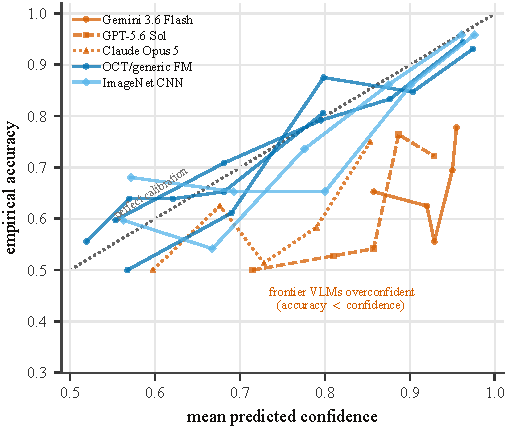
\includegraphics[width=0.55\linewidth]{figures/figA3_reliability.pdf}
  \caption{\textbf{Reliability diagram} (B-scan axis, few-shot), one line per configuration: empirical accuracy vs.\ mean
  predicted confidence in five equal-count bins for readability (dotted = perfect calibration; the ECE metric
  itself uses 10 equal-width bins, \S\ref{app:setup}). Every frontier VLM
  (Gemini 3.6 Flash, GPT-5.6 Sol, Claude Opus~5; one warm color, distinguished by line style) lies below the diagonal
  (overconfident), most for Gemini and least for Claude, whereas the OCT/generic FMs and ImageNet CNNs (cool
  colors) track it (well-calibrated).}
  \label{fig:reliability}
\end{figure}

\paragraph{Net calibration error and post-hoc calibration.} The miscalibration is directional and largely fixable
post hoc, yet the decision failure is not. For each frontier configuration we compute the net calibration error
(NCE), a signed calibration error \citep{groot2024overconfidence}: mean decision-confidence ($\max(p,1{-}p)$) minus
decision accuracy on clean eyes (positive $=$ overconfident; the opposite sign to Groot et al.'s
accuracy$-$confidence convention). (The ECE in Table~\ref{tab:main} is instead the
referral-probability, or positive-class, calibration error; the NCE and the reliability diagram use the
predicted-class confidence $\max(p,1{-}p)$. Both show the frontier VLMs are badly miscalibrated.) The Gemini and GPT
configurations have NCE \num{0.23}--\num{0.42} (few-shot \num{0.23}--\num{0.32}, zero-shot up to \num{0.42}); Claude
Opus~5 is far smaller (\num{0.08}--\num{0.13}), matching the diagram ordering above.
Post-hoc temperature scaling \citep{guo2017calibration} (one scalar fit on a held-out clean half by minimizing NLL)
removes most of the clean ECE (on the held-out clean half: Gemini 3.6 Flash few-shot \num{0.27}$\rightarrow$\num{0.07},
GPT-5.6 Sol \num{0.26}$\rightarrow$\num{0.07}), but, being strictly monotone, it preserves the score ordering and
fixes the $0.5$ decision point, so the decision-flip is exactly unchanged (and the refit 90\%-specificity operating
point selects the same decisions). Calibration is a post-hoc fix; the
scanner-driven decision-flip is not.

\paragraph{Calibration beyond fixed-bin ECE.} Fixed-bin ECE is a biased estimator at $n{\approx}300$--$360$ and
depends on the binning scheme, so we recompute the clean-eye calibration under two complementary reads with different
failure modes: adaptive (equal-count) ECE, which debiases the fixed binning, and the Brier score, a strictly proper
scoring rule with no binning (the proper-score check used under dataset shift by \citet{ovadia2019shift}). Both are
reported for every reader on both axes as extra columns in the full tables (App.~\ref{app:fulltables}). The frontier
VLMs stay worse than every FM/CNN reader on all three reads (fixed-bin ECE, adaptive ECE, and Brier; Claude Opus~5 the
least-overconfident exception), so the overconfidence gap is not an artifact of the ECE binning.

\section{Shift calibration and real-data corroboration}
\label{app:validity}

The synthetic shift is magnitude-tied to the published cross-scanner agreement literature and direction-corroborated
by real data. \emph{Thickness-map axis:} the Cirrus$\rightarrow$Spectralis RNFL offset reproduces
\citet{warner2011loa}'s $+1.94\,\mu$m bias and $\pm7.68\,\mu$m 95\% limits (difference SD $3.92\,\mu$m,
Fig.~\ref{fig:a1}a, a Bland--Altman plot \citep{blandaltman1986}). The per-eye spread is anatomy-coupled, drawn in
quadrature from segmentation, centration, and magnification mechanisms (between-eye SDs $2.8/2.3/1.5\,\mu$m) with
superior/inferior-wider sector gains, so limits widen in the vulnerable sectors (Fig.~\ref{fig:a1}b). The magnitude
is calibrated to Warner's Bland--Altman statistics, and the superior/inferior-wider spatial profile follows the
dominant cross-device error mechanism, scan-circle centration, which perturbs the superior and inferior sectors most
\citep{cheung2009scancircle}; the three mechanism components sum in quadrature to the published SD by construction,
so both the shift magnitude and its sector direction are anchored in measured cross-scanner data and established
optics. The finer within-eye texture is a small mean-zero term for spatially-correlated segmentation differences, which
are largest in the superior and inferior sectors \citep{mansberger2017segerrors}. This smoothness is data-driven: the real cross-vendor cpRNFL difference
(GLEAM Spectralis vs GOALS Topcon) is itself spatially smooth, with $74\%$ of its angular variance
in the lowest five harmonics and a $\sim$$22^{\circ}$ correlation length (roughness $0.79$ vs $1.41$ for white
noise), i.e.\ a low-frequency difference, not per-pixel noise. Being mean-zero, the texture leaves the calibrated
between-eye bias and LoA intact; these are validated directly by the Bland--Altman fit (Fig.~\ref{fig:a1}a) and the
monotone dose--response (Fig.~\ref{fig:a1}c), so Fig.~\ref{fig:overview}'s difference panels illustrate the
calibrated shift rather than assert a per-pixel measurement. Decision-flip and read-drift rise monotonically with dose (Fig.~\ref{fig:a1}c). \emph{B-scan axis:} the
Spectralis$\rightarrow$Topcon stress changes frame-averaging (16$\rightarrow$1 frames), injects a
multiplicative-Gamma speckle field that lifts display-speckle contrast $0.148\rightarrow0.184$ (matched to real
RETOUCH, Fig.~\ref{fig:a2}a), adds near-inert axial blur ($\sqrt{15}\,\mu$m FWHM at $10\,\mu$m/px), and dims
backscatter contrast $\times0.773$. Real cross-vendor cpRNFL corroborates that disc anatomy is vendor-consistent:
with a single segmenter \citep{driessen2024}, cpRNFL profiles from GLEAM Spectralis and GOALS Topcon
\citep{goals2022} B-scans agree in shape ($r\approx0.93$, Fig.~\ref{fig:a2}b). This corroborates that the scanner
perturbs the measurement, not the anatomy; it is a shape agreement, not a claim of scanner-interchangeability.

\begin{figure}[tbp]
  \centering
  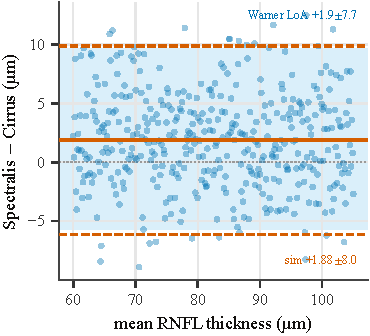
\includegraphics[width=0.32\linewidth]{figures/figA1a_bland_altman.pdf}\hfill
  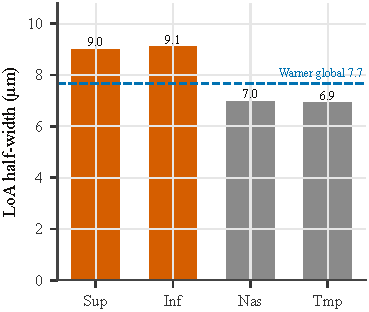
\includegraphics[width=0.32\linewidth]{figures/figA1b_sector_loa.pdf}\hfill
  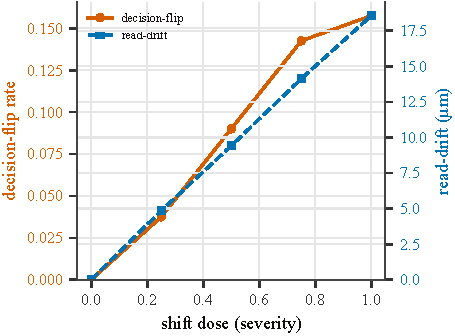
\includegraphics[width=0.32\linewidth]{figures/figA1c_dose_response.pdf}
  \caption{\textbf{Thickness-map shift is LoA-calibrated.} (a)~Bland--Altman of the synthetic per-eye differences
  against Warner's published 95\% limits (band); (b)~limits widen in the superior/inferior sectors;
  (c)~decision-flip and read-drift rise monotonically with shift dose, a graded axis rather than a cliff.}
  \label{fig:a1}
\end{figure}

\begin{figure}[tbp]
  \centering
  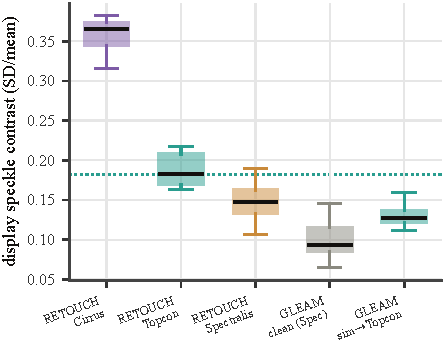
\includegraphics[width=0.44\linewidth]{figures/figA2a_speckle.pdf}\hfill
  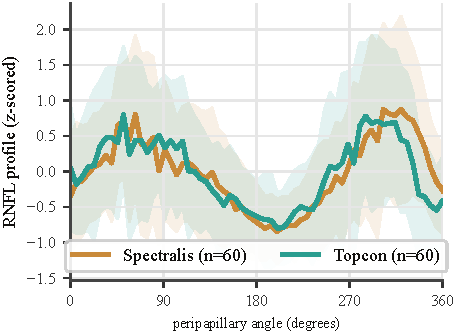
\includegraphics[width=0.44\linewidth]{figures/figA2b_crossvendor.pdf}
  \caption{\textbf{Appearance/anatomy validity.} (a)~Real per-vendor RETOUCH display speckle (Cirrus $>$ Topcon $>$
  Spectralis) validates the frame-averaging direction and the calibrated sim moves GLEAM toward Topcon;
  (b)~real cross-vendor cpRNFL: GLEAM Spectralis vs.\ GOALS Topcon profiles (single segmenter) agree in shape
  ($r\approx0.93$; shape only, not device-interchangeability).}
  \label{fig:a2}
\end{figure}

\section{Thickness-map vs.\ raw-B-scan reading, per VLM (F2)}
\label{app:grounding}
Fig.~\ref{fig:grounding} details F2. Rendering the same eye as a color thickness map instead of a raw B-scan raises
each stronger frontier VLM into the non-VLM reader band on discrimination and pulls it down on ECE and decision-flip
together, while the small open/specialist VLMs do not recover. This is a cross-dataset comparison (the two axes use
different datasets, vendors and label sources), so we read it as reader-specific, not as evidence that a thickness
map is intrinsically a better input (\S\ref{sec:discussion}).

\begin{figure}[tbp]
  \centering
  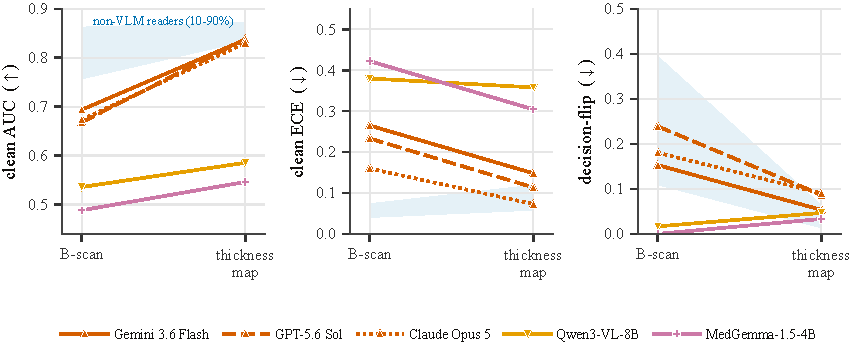
\includegraphics[width=0.72\linewidth]{figures/figA4_grounding.pdf}
  \caption{\textbf{The per-VLM thickness-map improvement, in three metrics.} Per-VLM change from the raw B-scan to the color
  thickness-map render (few-shot); the three frontier VLMs share the vermilion triangle and are distinguished by
  line style. The stronger frontier VLMs rise into the per-axis non-VLM reader band (10--90th percentile of the FM
  and CNN readers) on clean AUC and descend toward it on ECE and decision-flip together. The small open
  (Qwen3-VL-8B) and specialist (MedGemma-1.5-4B) models do not recover.}
  \label{fig:grounding}
\end{figure}

\section{Subgroup robustness}
\label{app:subgroups}
We ask whether the scanner-induced instability falls unevenly across disease severity or demographics, recomputing
decision-flip per subgroup for every configuration on the seed-0 test split
(\texttt{scripts/analyze\_subgroups.py}). Fig.~\ref{fig:subgroups} aggregates this by the four
capable reader classes (class mean and across-model spread; the near-chance open/specialist VLMs are near-constant and
omitted from the figure), and Tables~\ref{tab:sev}--\ref{tab:demo} give the per-reader point estimates for all
configurations. Decision-flip stays broadly comparable across subgroups. No severity grade or demographic group
shows a consistently elevated flip once the wide eye-level bootstrap CIs are accounted for. The one clear pattern is the B-scan over-referral of \S\ref{sec:findings}: for the appearance-keyed
readers the \emph{healthy} eyes flip most (MIRAGE\,$\cdot$\,LP \num{0.62} vs.\ \num{0.28} moderate/advanced; RETFound\,$\cdot$\,LP
\num{0.47} vs.\ \num{0.09}; SmallCNN \num{0.35} vs.\ \num{0.15}), i.e.\ the false-referral load concentrates in the
screening-relevant non-glaucoma population. Sensitivity change ($\Delta$sens) is likewise small and CI-overlapping
across the glaucoma severity subgroups. \emph{Caveats}: the GLEAM severity subgroups are small ($n\approx 57$--$184$ per
grade, so 95\% CIs span $\approx\pm0.08$--$0.13$); \textbf{image quality is not recorded in either dataset} and GLEAM
carries no demographics, so those subgroup axes cannot be tested and are left to future work.

\begin{figure}[tbp]
  \centering
  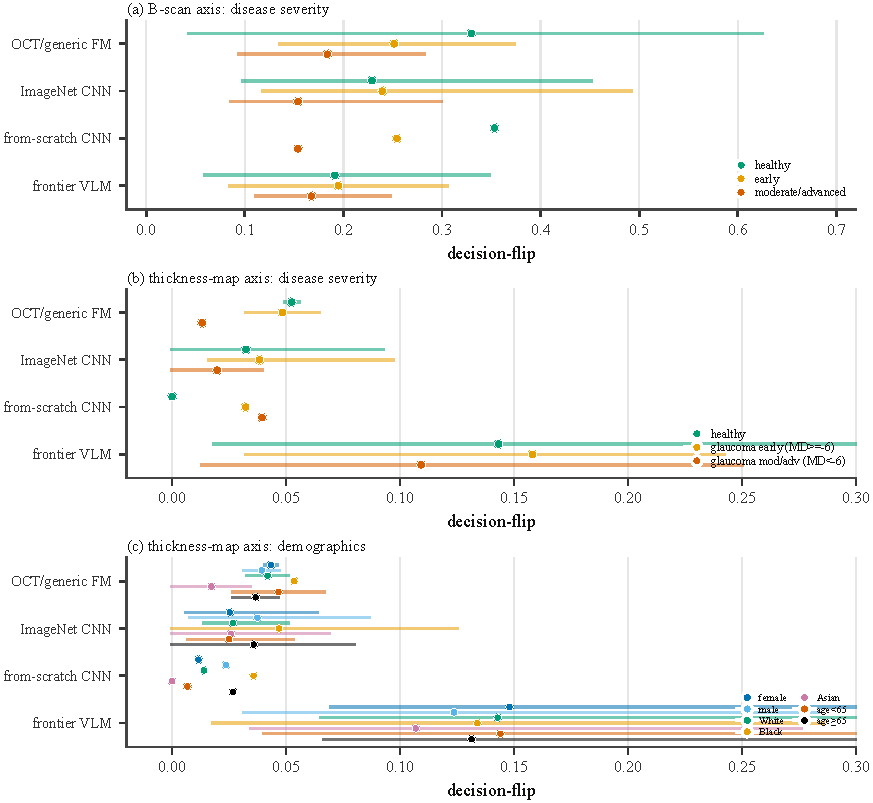
\includegraphics[width=0.86\linewidth]{figures/figA5_subgroups.pdf}
  \caption{\textbf{Decision-flip by subgroup, aggregated by reader class} (the four capable Fig.~\ref{fig:stability}
  classes; the near-constant open/specialist VLMs are omitted here but listed in Tables~\ref{tab:sev}--\ref{tab:demo}).
  Markers are the class mean across its models; bars span the min--max across those models. \textbf{(a)}~B-scan
  disease severity: for the appearance-keyed classes (OCT/generic FM, ImageNet CNN, from-scratch CNN) the healthy-eye
  flip is highest (over-referral on the screening population; the wide bars are within-class model spread, e.g.\ robust
  DINOv2\,$\cdot$\,FT vs.\ unstable MIRAGE\,$\cdot$\,LP), whereas the frontier VLMs are flat. \textbf{(b)}~Thickness-map
  severity and \textbf{(c)}~map demographics: flip stays low and the subgroups cluster for every class, with no group
  consistently elevated. The flip scale differs between (a) and (b,c).}
  \label{fig:subgroups}
\end{figure}

% auto-generated by scripts/build_paper_tables.py — do not edit by hand
\begin{table}[tbp]
  \centering
  \caption{\textbf{Decision-flip by disease severity}, both axes, all configurations (point estimates; the per-reader eye-level bootstrap 95\% CIs are wide and overlapping across grades, and the class-aggregated means and model spread are in Fig.~\ref{fig:subgroups}a,b). Severity: B-scan from the GLEAM 4-class label (healthy / early / moderate-advanced); map from Harvard-GDP mean deviation (healthy / MD$\ge-6$ / MD$<-6$). ``--'' = reader not run on that axis.}
  \label{tab:sev}
  \small
  \renewcommand{\arraystretch}{0.9}
  \setlength{\tabcolsep}{5pt}
  \begin{tabular}{lcccccc}
    \toprule
    & \multicolumn{3}{c}{B-scan axis} & \multicolumn{3}{c}{Thickness-map axis} \\
    \cmidrule(lr){2-4}\cmidrule(lr){5-7}
    Reader & healthy & early & mod/adv & healthy & early & mod/adv \\
    \midrule
    DINOv2\,$\cdot$\,FT & 0.04 & 0.14 & 0.13 & 0.05 & 0.03 & 0.01 \\
    DINOv2\,$\cdot$\,LP & 0.18 & 0.14 & 0.24 & 0.06 & 0.06 & 0.01 \\
    MIRAGE\,$\cdot$\,FT & 0.51 & 0.34 & 0.25 & -- & -- & -- \\
    MIRAGE\,$\cdot$\,LP & 0.62 & 0.37 & 0.28 & -- & -- & -- \\
    RETFound\,$\cdot$\,FT & 0.15 & 0.17 & 0.11 & -- & -- & -- \\
    RETFound\,$\cdot$\,LP & 0.47 & 0.36 & 0.09 & -- & -- & -- \\
    ConvNeXt-B\,$\cdot$\,FT & 0.16 & 0.15 & 0.09 & 0.00 & 0.02 & 0.03 \\
    ConvNeXt-B\,$\cdot$\,LP & 0.10 & 0.15 & 0.09 & 0.02 & 0.02 & 0.00 \\
    ConvNeXt-L\,$\cdot$\,FT & 0.18 & 0.19 & 0.09 & 0.01 & 0.03 & 0.03 \\
    ConvNeXt-L\,$\cdot$\,LP & 0.17 & 0.19 & 0.15 & 0.04 & 0.06 & 0.01 \\
    ConvNeXt-T\,$\cdot$\,FT & 0.12 & 0.12 & 0.09 & 0.02 & 0.02 & 0.00 \\
    ConvNeXt-T\,$\cdot$\,LP & 0.41 & 0.37 & 0.16 & 0.01 & 0.03 & 0.03 \\
    ResNet-50\,$\cdot$\,FT & 0.45 & 0.49 & 0.26 & 0.09 & 0.03 & 0.03 \\
    ResNet-50\,$\cdot$\,LP & 0.23 & 0.25 & 0.30 & 0.06 & 0.10 & 0.04 \\
    SmallCNN (98k) & 0.35 & 0.25 & 0.15 & 0.00 & 0.03 & 0.04 \\
    Claude Opus~5\,\textit{fs} & 0.23 & 0.17 & 0.11 & 0.10 & 0.11 & 0.04 \\
    Claude Opus~5\,\textit{zs} & 0.35 & 0.24 & 0.16 & 0.03 & 0.18 & 0.08 \\
    GPT-5.6 Sol\,\textit{fs} & 0.21 & 0.31 & 0.25 & 0.10 & 0.10 & 0.04 \\
    GPT-5.6 Sol\,\textit{zs} & 0.06 & 0.08 & 0.11 & 0.02 & 0.16 & 0.18 \\
    Gemini 2.5 Flash\,\textit{fs} & 0.20 & 0.29 & 0.19 & 0.30 & 0.23 & 0.09 \\
    Gemini 2.5 Flash\,\textit{zs} & 0.10 & 0.12 & 0.11 & 0.37 & 0.19 & 0.25 \\
    Gemini 2.5 Pro\,\textit{fs} & 0.27 & 0.19 & 0.21 & 0.17 & 0.18 & 0.09 \\
    Gemini 2.5 Pro\,\textit{zs} & 0.12 & 0.17 & 0.14 & 0.24 & 0.24 & 0.18 \\
    Gemini 3.6 Flash\,\textit{fs} & 0.14 & 0.20 & 0.15 & 0.08 & 0.03 & 0.01 \\
    Gemini 3.6 Flash\,\textit{zs} & 0.23 & 0.19 & 0.25 & 0.02 & 0.16 & 0.12 \\
    Qwen3-VL-8B\,\textit{fs} & 0.02 & 0.02 & 0.01 & 0.07 & 0.02 & 0.01 \\
    Qwen3-VL-8B\,\textit{zs} & 0.21 & 0.17 & 0.15 & 0.01 & 0.00 & 0.00 \\
    MedGemma-1.5-4B\,\textit{fs} & 0.00 & 0.00 & 0.00 & 0.02 & 0.08 & 0.01 \\
    MedGemma-1.5-4B\,\textit{zs} & 0.00 & 0.00 & 0.00 & 0.02 & 0.03 & 0.00 \\
    \bottomrule
  \end{tabular}
\end{table}

\begin{table}[tbp]
  \centering
  \caption{\textbf{Decision-flip by demographics} (thickness-map axis, Harvard-GDP; all configurations, point estimates, wide overlapping CIs; class-aggregated view in Fig.~\ref{fig:subgroups}c). No group is consistently elevated. GLEAM (B-scan) carries no demographics.}
  \label{tab:demo}
  \small
  \renewcommand{\arraystretch}{0.9}
  \setlength{\tabcolsep}{5pt}
  \begin{tabular}{lccccccc}
    \toprule
    & \multicolumn{2}{c}{gender} & \multicolumn{3}{c}{race} & \multicolumn{2}{c}{age} \\
    \cmidrule(lr){2-3}\cmidrule(lr){4-6}\cmidrule(lr){7-8}
    Reader & F & M & White & Black & Asian & $<$65 & $\ge$65 \\
    \midrule
    DINOv2\,$\cdot$\,FT & 0.04 & 0.03 & 0.03 & 0.05 & 0.03 & 0.03 & 0.05 \\
    DINOv2\,$\cdot$\,LP & 0.05 & 0.05 & 0.05 & 0.05 & 0.00 & 0.07 & 0.03 \\
    ConvNeXt-B\,$\cdot$\,FT & 0.01 & 0.01 & 0.01 & 0.00 & 0.00 & 0.02 & 0.00 \\
    ConvNeXt-B\,$\cdot$\,LP & 0.01 & 0.02 & 0.02 & 0.00 & 0.00 & 0.01 & 0.01 \\
    ConvNeXt-L\,$\cdot$\,FT & 0.01 & 0.02 & 0.01 & 0.04 & 0.00 & 0.01 & 0.03 \\
    ConvNeXt-L\,$\cdot$\,LP & 0.03 & 0.05 & 0.04 & 0.04 & 0.07 & 0.03 & 0.05 \\
    ConvNeXt-T\,$\cdot$\,FT & 0.01 & 0.02 & 0.01 & 0.04 & 0.00 & 0.01 & 0.02 \\
    ConvNeXt-T\,$\cdot$\,LP & 0.02 & 0.02 & 0.02 & 0.02 & 0.03 & 0.01 & 0.03 \\
    ResNet-50\,$\cdot$\,FT & 0.06 & 0.06 & 0.05 & 0.12 & 0.07 & 0.05 & 0.08 \\
    ResNet-50\,$\cdot$\,LP & 0.05 & 0.09 & 0.05 & 0.12 & 0.03 & 0.05 & 0.07 \\
    SmallCNN (98k) & 0.01 & 0.02 & 0.01 & 0.04 & 0.00 & 0.01 & 0.03 \\
    Claude Opus~5\,\textit{fs} & 0.11 & 0.06 & 0.08 & 0.11 & 0.10 & 0.09 & 0.09 \\
    Claude Opus~5\,\textit{zs} & 0.08 & 0.07 & 0.07 & 0.11 & 0.03 & 0.08 & 0.07 \\
    GPT-5.6 Sol\,\textit{fs} & 0.11 & 0.06 & 0.08 & 0.11 & 0.07 & 0.10 & 0.07 \\
    GPT-5.6 Sol\,\textit{zs} & 0.09 & 0.09 & 0.08 & 0.14 & 0.03 & 0.09 & 0.09 \\
    Gemini 2.5 Flash\,\textit{fs} & 0.25 & 0.20 & 0.22 & 0.23 & 0.28 & 0.24 & 0.22 \\
    Gemini 2.5 Flash\,\textit{zs} & 0.32 & 0.28 & 0.33 & 0.29 & 0.17 & 0.30 & 0.31 \\
    Gemini 2.5 Pro\,\textit{fs} & 0.16 & 0.14 & 0.17 & 0.12 & 0.07 & 0.19 & 0.11 \\
    Gemini 2.5 Pro\,\textit{zs} & 0.24 & 0.21 & 0.26 & 0.14 & 0.17 & 0.25 & 0.20 \\
    Gemini 3.6 Flash\,\textit{fs} & 0.07 & 0.03 & 0.07 & 0.02 & 0.03 & 0.04 & 0.07 \\
    Gemini 3.6 Flash\,\textit{zs} & 0.07 & 0.08 & 0.07 & 0.07 & 0.10 & 0.07 & 0.08 \\
    Qwen3-VL-8B\,\textit{fs} & 0.06 & 0.03 & 0.05 & 0.05 & 0.03 & 0.07 & 0.03 \\
    Qwen3-VL-8B\,\textit{zs} & 0.00 & 0.01 & 0.00 & 0.00 & 0.00 & 0.01 & 0.00 \\
    MedGemma-1.5-4B\,\textit{fs} & 0.03 & 0.04 & 0.03 & 0.05 & 0.03 & 0.03 & 0.03 \\
    MedGemma-1.5-4B\,\textit{zs} & 0.03 & 0.01 & 0.01 & 0.00 & 0.10 & 0.03 & 0.01 \\
    \bottomrule
  \end{tabular}
\end{table}


\section{Full per-axis tables}
\label{app:fulltables}
% auto-generated by scripts/build_paper_tables.py — do not edit by hand
\begin{table}[h]
  \centering
  \caption{\textbf{Full B-scan (appearance) axis, all 29 configurations}. Spectralis\,$\rightarrow$\,Topcon speckle shift ($n{=}360$ eyes). spec@shift = realized specificity under the shift at the 90\%-specificity operating point (a low value signals decision collapse); ECE, aECE and Brier have no bootstrap CI in the released summaries. ECE is the positive-class calibration error (10 equal-width bins); aECE is the adaptive (equal-mass) ECE and Brier is the Brier score, a strictly proper score with no binning, so together they show the calibration reads are not a fixed-bin artifact. NCE $=$ net calibration error, a signed calibration error \citep{groot2024overconfidence} (mean predicted-class confidence minus accuracy; $+$ $=$ overconfident). All calibration reads are on the clean eyes.}
  \small
  \setlength{\tabcolsep}{3pt}
  \resizebox{\linewidth}{!}{%
  \begin{tabular}{llccccccccc}
    \toprule
    Reader & Class & AUC \ci{95\%}{CI} & Flip \ci{95\%}{CI} & $\Delta$sens \ci{95\%}{CI} & spec@shift & ECE & aECE & Brier & NCE & $\Delta$AUC \\
    \midrule
    DINOv2\,$\cdot$\,FT & FM & 0.876 \ci{0.84}{0.91} & 0.086 \ci{0.06}{0.12} & +0.080 \ci{0.03}{0.13} & 0.92 & 0.052 & 0.073 & 0.145 & -0.003 & +0.011 \\
    RETFound\,$\cdot$\,FT & FM & 0.847 \ci{0.80}{0.89} & 0.142 \ci{0.11}{0.18} & -0.091 \ci{-0.14}{-0.04} & 0.81 & 0.072 & 0.080 & 0.158 & +0.067 & -0.007 \\
    RETFound\,$\cdot$\,LP & FM & 0.845 \ci{0.80}{0.88} & 0.328 \ci{0.28}{0.38} & -0.227 \ci{-0.29}{-0.16} & 0.52 & 0.040 & 0.035 & 0.160 & -0.001 & +0.061 \\
    DINOv2\,$\cdot$\,LP & FM & 0.842 \ci{0.80}{0.88} & 0.194 \ci{0.16}{0.24} & +0.165 \ci{0.10}{0.23} & 0.92 & 0.047 & 0.039 & 0.162 & +0.034 & +0.059 \\
    MIRAGE\,$\cdot$\,FT & FM & 0.736 \ci{0.68}{0.78} & 0.394 \ci{0.34}{0.44} & -0.386 \ci{-0.46}{-0.32} & 0.61 & 0.121 & 0.119 & 0.220 & +0.097 & -0.002 \\
    MIRAGE\,$\cdot$\,LP & FM & 0.701 \ci{0.65}{0.76} & 0.472 \ci{0.42}{0.52} & -0.722 \ci{-0.79}{-0.65} & 0.07 & 0.041 & 0.067 & 0.221 & -0.021 & +0.044 \\
    ConvNeXt-T\,$\cdot$\,FT & ImageNet CNN & 0.869 \ci{0.83}{0.90} & 0.111 \ci{0.08}{0.14} & -0.097 \ci{-0.14}{-0.06} & 0.68 & 0.067 & 0.070 & 0.147 & -0.003 & +0.026 \\
    ConvNeXt-B\,$\cdot$\,FT & ImageNet CNN & 0.854 \ci{0.81}{0.89} & 0.136 \ci{0.10}{0.17} & -0.051 \ci{-0.10}{0.01} & 0.74 & 0.049 & 0.067 & 0.155 & -0.019 & +0.050 \\
    ConvNeXt-L\,$\cdot$\,FT & ImageNet CNN & 0.836 \ci{0.79}{0.87} & 0.153 \ci{0.12}{0.19} & -0.068 \ci{-0.12}{-0.02} & 0.76 & 0.066 & 0.067 & 0.164 & +0.051 & +0.045 \\
    ResNet-50\,$\cdot$\,FT & ImageNet CNN & 0.833 \ci{0.78}{0.87} & 0.394 \ci{0.34}{0.44} & -0.307 \ci{-0.37}{-0.24} & 0.55 & 0.068 & 0.078 & 0.169 & +0.035 & +0.006 \\
    ConvNeXt-B\,$\cdot$\,LP & ImageNet CNN & 0.826 \ci{0.78}{0.87} & 0.108 \ci{0.07}{0.14} & +0.068 \ci{0.02}{0.13} & 0.91 & 0.070 & 0.055 & 0.170 & +0.029 & +0.038 \\
    ConvNeXt-T\,$\cdot$\,LP & ImageNet CNN & 0.826 \ci{0.78}{0.87} & 0.325 \ci{0.28}{0.38} & -0.199 \ci{-0.26}{-0.14} & 0.60 & 0.036 & 0.051 & 0.169 & +0.031 & +0.038 \\
    ConvNeXt-L\,$\cdot$\,LP & ImageNet CNN & 0.825 \ci{0.78}{0.86} & 0.167 \ci{0.13}{0.21} & +0.028 \ci{-0.03}{0.09} & 0.83 & 0.062 & 0.058 & 0.168 & +0.014 & +0.048 \\
    ResNet-50\,$\cdot$\,LP & ImageNet CNN & 0.825 \ci{0.78}{0.86} & 0.258 \ci{0.22}{0.30} & +0.136 \ci{0.06}{0.21} & 0.89 & 0.075 & 0.076 & 0.174 & +0.027 & +0.080 \\
    SmallCNN (98k) & scratch CNN & 0.788 \ci{0.74}{0.83} & 0.272 \ci{0.23}{0.32} & -0.324 \ci{-0.40}{-0.25} & 0.65 & 0.042 & 0.063 & 0.189 & -0.039 & +0.017 \\
    Gemini 3.6 Flash\,\textit{fs} & frontier VLM & 0.694 \ci{0.64}{0.74} & 0.153 \ci{0.12}{0.19} & +0.006 \ci{-0.03}{0.04} & 0.90 & 0.265 & 0.260 & 0.292 & +0.258 & -0.001 \\
    Claude Opus~5\,\textit{fs} & frontier VLM & 0.673 \ci{0.62}{0.73} & 0.181 \ci{0.14}{0.22} & +0.045 \ci{0.00}{0.09} & 0.97 & 0.160 & 0.159 & 0.253 & +0.132 & +0.030 \\
    GPT-5.6 Sol\,\textit{fs} & frontier VLM & 0.668 \ci{0.61}{0.73} & 0.239 \ci{0.19}{0.28} & +0.108 \ci{0.05}{0.17} & 0.92 & 0.233 & 0.218 & 0.283 & +0.228 & -0.012 \\
    Gemini 2.5 Pro\,\textit{fs} & frontier VLM & 0.635 \ci{0.58}{0.69} & 0.239 \ci{0.20}{0.28} & -0.017 \ci{-0.06}{0.02} & 0.99 & 0.324 & 0.313 & 0.338 & +0.322 & -0.004 \\
    GPT-5.6 Sol\,\textit{zs} & frontier VLM & 0.631 \ci{0.58}{0.69} & 0.081 \ci{0.06}{0.11} & +0.045 \ci{-0.02}{0.11} & 0.92 & 0.307 & 0.297 & 0.337 & +0.304 & -0.004 \\
    Gemini 2.5 Flash\,\textit{fs} & frontier VLM & 0.622 \ci{0.57}{0.68} & 0.211 \ci{0.17}{0.25} & +0.040 \ci{-0.01}{0.09} & 0.95 & 0.297 & 0.279 & 0.325 & +0.295 & +0.013 \\
    Claude Opus~5\,\textit{zs} & frontier VLM & 0.607 \ci{0.55}{0.66} & 0.269 \ci{0.22}{0.31} & -0.034 \ci{-0.09}{0.02} & 0.97 & 0.113 & 0.090 & 0.250 & +0.076 & +0.010 \\
    Gemini 3.6 Flash\,\textit{zs} & frontier VLM & 0.596 \ci{0.54}{0.65} & 0.228 \ci{0.19}{0.27} & -0.011 \ci{-0.08}{0.05} & 0.89 & 0.356 & 0.308 & 0.368 & +0.349 & +0.032 \\
    Gemini 2.5 Flash\,\textit{zs} & frontier VLM & 0.571 \ci{0.52}{0.62} & 0.108 \ci{0.08}{0.14} & +0.023 \ci{-0.03}{0.08} & 0.91 & 0.390 & 0.372 & 0.399 & +0.379 & +0.053 \\
    Gemini 2.5 Pro\,\textit{zs} & frontier VLM & 0.515 \ci{0.47}{0.56} & 0.133 \ci{0.10}{0.17} & +0.023 \ci{-0.04}{0.09} & 0.92 & 0.422 & 0.407 & 0.427 & +0.420 & -0.029 \\
    Qwen3-VL-8B\,\textit{fs} & open VLM & 0.536 \ci{0.49}{0.58} & 0.017 \ci{0.01}{0.03} & +0.000 \ci{0.00}{0.00} & 1.00 & 0.380 & 0.369 & 0.393 & +0.380 & +0.000 \\
    Qwen3-VL-8B\,\textit{zs} & open VLM & 0.462 \ci{0.42}{0.50} & 0.186 \ci{0.15}{0.23} & +0.000 \ci{0.00}{0.00} & 1.00 & 0.510 & 0.487 & 0.510 & +0.510 & +0.038 \\
    MedGemma-1.5-4B\,\textit{zs} & specialist VLM & 0.539 \ci{0.49}{0.58} & 0.000 \ci{0.00}{0.00} & +0.023 \ci{-0.01}{0.05} & 0.99 & 0.464 & 0.465 & 0.463 & +0.465 & -0.015 \\
    MedGemma-1.5-4B\,\textit{fs} & specialist VLM & 0.488 \ci{0.43}{0.54} & 0.000 \ci{0.00}{0.00} & +0.034 \ci{0.00}{0.07} & 0.98 & 0.422 & 0.422 & 0.430 & +0.422 & -0.036 \\
    \bottomrule
  \end{tabular}}
\end{table}

\begin{table}[h]
  \centering
  \caption{\textbf{Full thickness-map (color-map) axis, all 25 configurations}. Cirrus\,$\rightarrow$\,Spectralis offset; OCT-specific B-scan FMs are not run on map renders ($n{=}300$ eyes). spec@shift = realized specificity under the shift at the 90\%-specificity operating point (a low value signals decision collapse); ECE, aECE and Brier have no bootstrap CI in the released summaries. ECE is the positive-class calibration error (10 equal-width bins); aECE is the adaptive (equal-mass) ECE and Brier is the Brier score, a strictly proper score with no binning, so together they show the calibration reads are not a fixed-bin artifact. NCE $=$ net calibration error, a signed calibration error \citep{groot2024overconfidence} (mean predicted-class confidence minus accuracy; $+$ $=$ overconfident). All calibration reads are on the clean eyes.}
  \small
  \setlength{\tabcolsep}{3pt}
  \resizebox{\linewidth}{!}{%
  \begin{tabular}{llccccccccc}
    \toprule
    Reader & Class & AUC \ci{95\%}{CI} & Flip \ci{95\%}{CI} & $\Delta$sens \ci{95\%}{CI} & spec@shift & ECE & aECE & Brier & NCE & $\Delta$AUC \\
    \midrule
    DINOv2\,$\cdot$\,FT & FM & 0.876 \ci{0.83}{0.91} & 0.037 \ci{0.02}{0.06} & +0.014 \ci{-0.01}{0.04} & 0.93 & 0.090 & 0.089 & 0.136 & -0.018 & +0.004 \\
    DINOv2\,$\cdot$\,LP & FM & 0.849 \ci{0.80}{0.89} & 0.047 \ci{0.02}{0.07} & +0.029 \ci{-0.01}{0.07} & 0.90 & 0.078 & 0.062 & 0.153 & +0.035 & -0.001 \\
    ConvNeXt-L\,$\cdot$\,FT & ImageNet CNN & 0.872 \ci{0.83}{0.91} & 0.017 \ci{0.00}{0.03} & +0.007 \ci{-0.02}{0.03} & 0.91 & 0.067 & 0.074 & 0.137 & -0.040 & +0.001 \\
    ResNet-50\,$\cdot$\,FT & ImageNet CNN & 0.865 \ci{0.82}{0.91} & 0.063 \ci{0.04}{0.09} & +0.007 \ci{-0.02}{0.03} & 0.96 & 0.135 & 0.130 & 0.152 & -0.085 & -0.005 \\
    ConvNeXt-T\,$\cdot$\,FT & ImageNet CNN & 0.862 \ci{0.82}{0.91} & 0.017 \ci{0.00}{0.03} & +0.000 \ci{-0.03}{0.03} & 0.91 & 0.095 & 0.098 & 0.141 & -0.037 & -0.000 \\
    ConvNeXt-B\,$\cdot$\,FT & ImageNet CNN & 0.859 \ci{0.81}{0.90} & 0.010 \ci{0.00}{0.02} & +0.000 \ci{0.00}{0.00} & 0.91 & 0.112 & 0.169 & 0.170 & +0.011 & -0.001 \\
    ConvNeXt-B\,$\cdot$\,LP & ImageNet CNN & 0.843 \ci{0.79}{0.89} & 0.013 \ci{0.00}{0.03} & -0.014 \ci{-0.04}{0.01} & 0.90 & 0.057 & 0.065 & 0.151 & +0.021 & -0.001 \\
    ConvNeXt-T\,$\cdot$\,LP & ImageNet CNN & 0.836 \ci{0.79}{0.88} & 0.020 \ci{0.01}{0.04} & +0.058 \ci{0.02}{0.10} & 0.93 & 0.058 & 0.066 & 0.155 & +0.001 & -0.001 \\
    ConvNeXt-L\,$\cdot$\,LP & ImageNet CNN & 0.834 \ci{0.78}{0.88} & 0.040 \ci{0.02}{0.06} & -0.007 \ci{-0.03}{0.02} & 0.89 & 0.081 & 0.054 & 0.156 & +0.059 & -0.008 \\
    ResNet-50\,$\cdot$\,LP & ImageNet CNN & 0.831 \ci{0.78}{0.88} & 0.063 \ci{0.04}{0.09} & -0.007 \ci{-0.04}{0.03} & 0.88 & 0.058 & 0.067 & 0.163 & +0.029 & +0.014 \\
    SmallCNN (98k) & scratch CNN & 0.847 \ci{0.80}{0.89} & 0.017 \ci{0.00}{0.03} & +0.000 \ci{-0.04}{0.04} & 0.94 & 0.119 & 0.139 & 0.169 & +0.033 & -0.006 \\
    Claude Opus~5\,\textit{zs} & frontier VLM & 0.850 \ci{0.81}{0.89} & 0.073 \ci{0.05}{0.10} & +0.058 \ci{0.00}{0.12} & 0.93 & 0.106 & 0.113 & 0.167 & -0.011 & +0.023 \\
    GPT-5.6 Sol\,\textit{fs} & frontier VLM & 0.838 \ci{0.79}{0.88} & 0.087 \ci{0.06}{0.12} & +0.022 \ci{-0.03}{0.07} & 0.93 & 0.113 & 0.110 & 0.170 & +0.110 & -0.005 \\
    Gemini 3.6 Flash\,\textit{fs} & frontier VLM & 0.837 \ci{0.79}{0.88} & 0.053 \ci{0.03}{0.08} & +0.058 \ci{0.02}{0.09} & 0.93 & 0.148 & 0.140 & 0.175 & +0.134 & +0.016 \\
    Claude Opus~5\,\textit{fs} & frontier VLM & 0.830 \ci{0.78}{0.88} & 0.090 \ci{0.06}{0.12} & +0.029 \ci{-0.01}{0.07} & 0.93 & 0.073 & 0.074 & 0.161 & +0.014 & -0.002 \\
    Gemini 2.5 Pro\,\textit{fs} & frontier VLM & 0.807 \ci{0.76}{0.86} & 0.150 \ci{0.11}{0.19} & -0.051 \ci{-0.12}{0.01} & 0.96 & 0.150 & 0.153 & 0.189 & +0.150 & -0.007 \\
    Gemini 3.6 Flash\,\textit{zs} & frontier VLM & 0.797 \ci{0.75}{0.85} & 0.073 \ci{0.05}{0.10} & +0.043 \ci{-0.01}{0.11} & 0.94 & 0.230 & 0.226 & 0.239 & +0.201 & -0.006 \\
    Gemini 2.5 Flash\,\textit{fs} & frontier VLM & 0.775 \ci{0.72}{0.82} & 0.230 \ci{0.19}{0.28} & -0.029 \ci{-0.11}{0.04} & 0.94 & 0.173 & 0.147 & 0.218 & +0.169 & -0.001 \\
    GPT-5.6 Sol\,\textit{zs} & frontier VLM & 0.772 \ci{0.72}{0.82} & 0.090 \ci{0.06}{0.12} & -0.014 \ci{-0.09}{0.06} & 0.90 & 0.233 & 0.227 & 0.241 & +0.170 & -0.026 \\
    Gemini 2.5 Pro\,\textit{zs} & frontier VLM & 0.713 \ci{0.66}{0.77} & 0.227 \ci{0.18}{0.28} & -0.007 \ci{-0.09}{0.08} & 0.98 & 0.268 & 0.261 & 0.282 & +0.266 & +0.004 \\
    Gemini 2.5 Flash\,\textit{zs} & frontier VLM & 0.644 \ci{0.58}{0.71} & 0.303 \ci{0.26}{0.35} & +0.036 \ci{-0.03}{0.10} & 1.00 & 0.229 & 0.221 & 0.287 & +0.211 & -0.026 \\
    Qwen3-VL-8B\,\textit{fs} & open VLM & 0.585 \ci{0.55}{0.62} & 0.047 \ci{0.02}{0.07} & +0.000 \ci{-0.04}{0.04} & 0.94 & 0.358 & 0.345 & 0.369 & +0.358 & +0.018 \\
    Qwen3-VL-8B\,\textit{zs} & open VLM & 0.500 \ci{0.50}{0.50} & 0.003 \ci{0.00}{0.01} & +0.000 \ci{0.00}{0.00} & 1.00 & 0.490 & 0.490 & 0.489 & +0.490 & -0.003 \\
    MedGemma-1.5-4B\,\textit{fs} & specialist VLM & 0.546 \ci{0.48}{0.61} & 0.033 \ci{0.02}{0.06} & +0.000 \ci{-0.04}{0.04} & 0.92 & 0.304 & 0.291 & 0.341 & +0.299 & +0.025 \\
    MedGemma-1.5-4B\,\textit{zs} & specialist VLM & 0.411 \ci{0.35}{0.47} & 0.020 \ci{0.01}{0.04} & -0.014 \ci{-0.04}{0.00} & 0.95 & 0.384 & 0.364 & 0.406 & +0.379 & +0.018 \\
    \bottomrule
  \end{tabular}}
\end{table}


\section{Reproducibility and broader impact}
\label{app:repro}

\paragraph{Reproducibility.} We release the full pipeline, the verbatim prompts (\S\ref{app:prompts}), the per-configuration
model IDs and inference settings (Table~\ref{tab:models}), and all seeds. Splits are eye-level and seed-fixed;
encoder probes are fit on the seed-0 split; VLM elicitation is greedy (single sample). Because
frontier API models drift, we pin each model ID and API date and archive the raw per-eye model responses, so every
table and figure reproduces exactly from the released code and responses; re-querying a live API may differ as the
served model changes. On acceptance we release, under the MIT license, the exact synthetic-shift transforms (the
B-scan appearance transform and the thickness-map scanner-offset, with every parameter and per-eye seed) together
with the committed per-eye outputs, so a new model can be scored directly against the calibrated shift; the
datasets remain under their own access terms (GLEAM; Harvard-GDP CC BY-NC-ND 4.0; GOALS; RETOUCH).

\paragraph{Broader impact.} The deployment-relevant finding is a safety one: a reader can preserve AUC under
a scanner change while its diagnostic decisions flip, so a naive AUC-only validation can
license an unsafe glaucoma-diagnosis reader. We advocate decision-level, calibration-aware, shift-aware evaluation
before deployment, and release the benchmark as a reusable check. The study uses de-identified public research
datasets; no new patient data were collected.
